\graphicspath{{./figures}}

\section{Ground Station Antenna}
\subsection{Mechanical Integration}

The existing antennna mount is shown in Figure \ref{fig:antennaMount}. Azimuthal and elevation stepper motors are connected directly through Gear A and B respectively. Gear A rotates the centre shaft to provide azimuthal steering, whereas Gear B rotates through Gear D and E to allow a change in elevation (pointing angle).

The black plastic platform is triangular and has three mounting holes. The new ground station's antenna should therefore be mounted onto this platform. It is important to consider the forces/torques involved, as well as the stepper motor holding torques, in order to determine the maximum weight and acceptable form factor of the new antenna.

\begin{figure}[!htb]
  \centering
  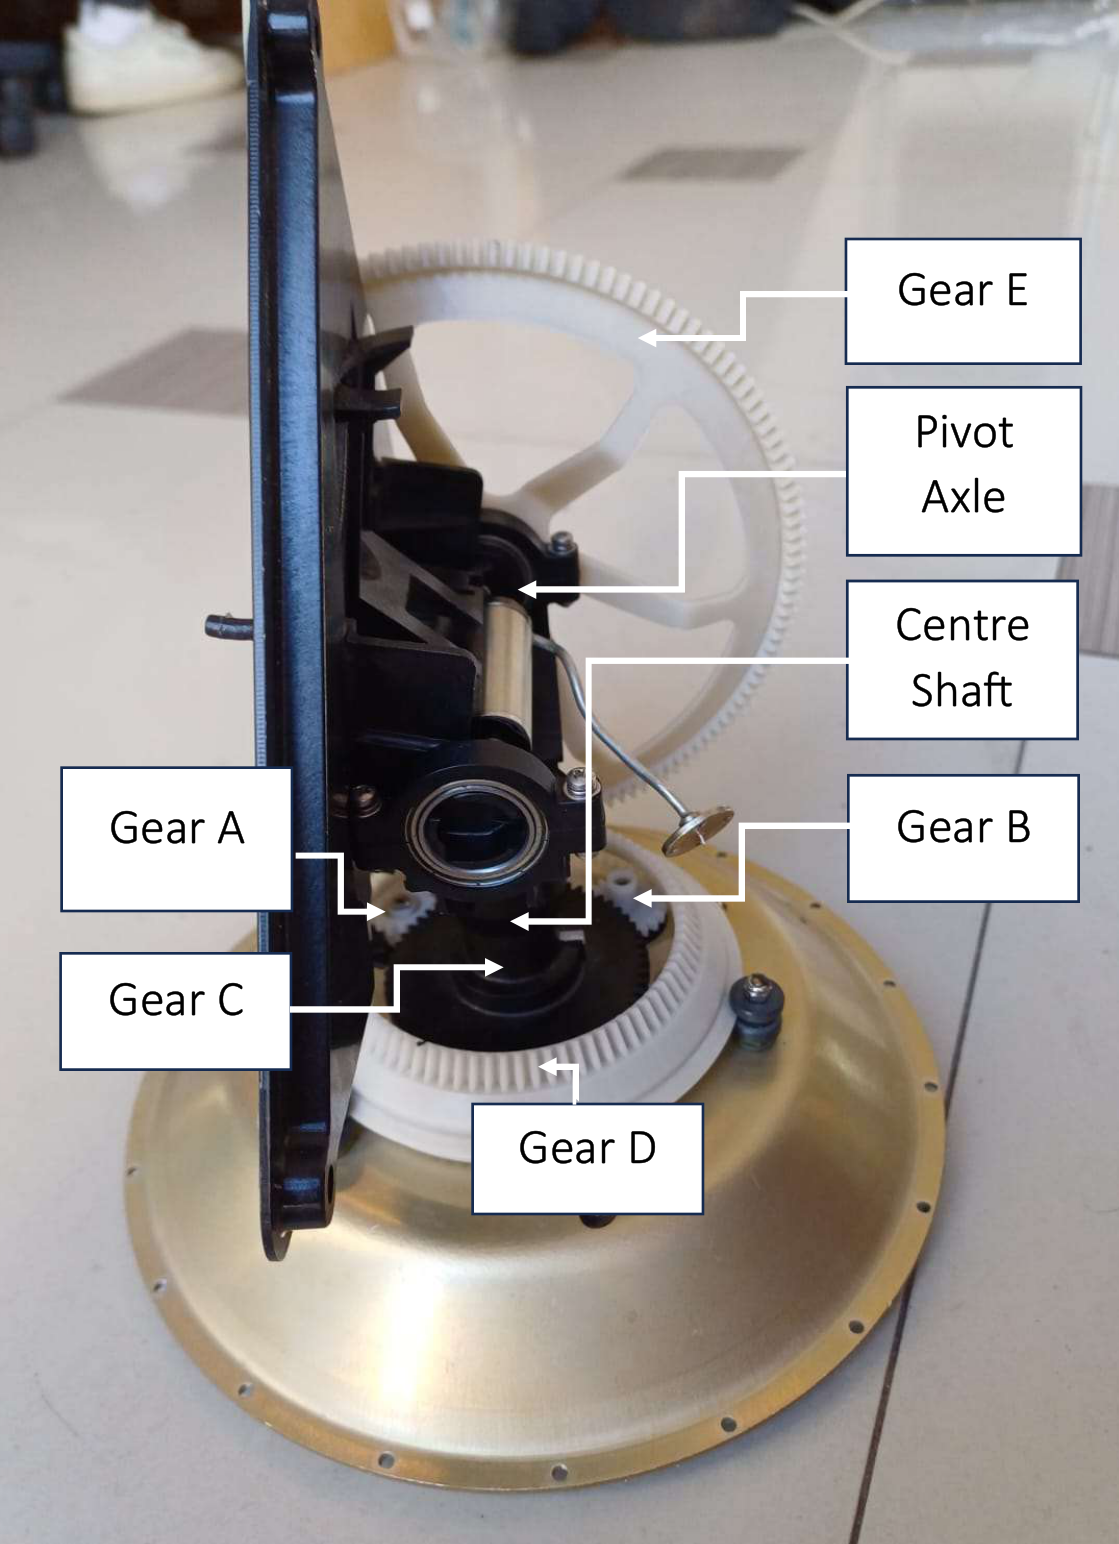
\includegraphics[width=0.35\textwidth]{antennaMount}
  \caption{The existing Antenna mount}
  \label{fig:antennaMount}
\end{figure}

Motors: 200 steps (full stepping)
Motors: 400 steps (half stepping)
Gear A: 15 teeth
Gear B: 20 teeth
Gear C: 60 teeth
Gear D: 92 teeth
Gear E: 140 teeth eq.

A-C-D
B-D-C

D/B = 4
C/A = 4
D/C = 1.33

C/A = 4
D/B = 4.6
D/C = 1.533
B/C = D/C * B/D =  1.5333 * 1/4.6 = 0.333
B/A = B/C * C/A = 0.333 * 4 = 





a -> 15 -> 60 -> 80        =      b -> 20 -> 92
80/60 * 60/15 * 15/a       = 92/20 * 20/b
80/a                       = 92/b
80/92 = a/b




Experimental 260.0/200.0 = 1.3
Actual = 1.333

The azimuthal motor need not be considered, as all torques from the mount to its base are perpendicular to the central shaft. The holding torque of the elevation motor, however, will constraint the antenna design. The holding torque of each motor is 0.25 Nm. The gearing ratio resulting from Gear B having 20 teeth, Gear D having 80 teeth, and finally Gear E having an equivalent of 140 teeth, results in a 7x torque increase. This provides a holding torque of around 1.75 Nm at the pivot axle.

The centre of gravity of the antenna, as well as its weight, will affect the motor's ability to hold it in place. The horizontal distance between the pivot axle and the mount in the upright position is measured to be 40mm. Therefore, in the worst-case (when the mount is upright as in Figure \ref{fig:antennaMount}) a planar antenna could weigh up to $\frac{1.75}{(9.8 \times 0.04)} = \SI{4.46}{kg}$. In general, the \textit{mass-distance} factor of the antenna (mass times distance of centre of gravity from mount) should not be more than 0.18 kg.m, which will be more limiting for protruding antennas.